% ===================================================================
%  Week 14 — Object Detection & Localization
%  Session 1 of 2: From "what" to "where" — boxes, sliding windows, IoU, NMS
%  Compile: pdflatex -interaction=nonstopmode slides-a.tex  (twice)
% ===================================================================
\documentclass[10pt,aspectratio=169]{beamer}
% ===================================================================
%  Shared Beamer preamble for "Practical Image Processing"
%  English slides. Compile with pdfLaTeX.
% ===================================================================

\usetheme{metropolis}
\usepackage[T1]{fontenc}
\usepackage[utf8]{inputenc}
\usepackage{lmodern}
\usepackage{listings}
\usepackage{tcolorbox}
\usepackage{fontawesome5}
\usepackage{booktabs}
\usepackage{amsmath,amssymb}
\usepackage{tikz}
\usepackage{pgfplots}
\pgfplotsset{compat=1.17}
\usetikzlibrary{arrows.meta,positioning,shapes.geometric,fit,backgrounds,matrix}
\tcbuselibrary{skins,breakable}

% ---- Palette --------------------------------------------------------
\definecolor{coursePrimary}{HTML}{1B4965}   % deep blue
\definecolor{courseAccent}{HTML}{E76F51}    % coral
\definecolor{courseGood}{HTML}{2A9D8F}      % teal
\definecolor{courseBad}{HTML}{C0392B}       % red
\definecolor{courseInfo}{HTML}{2980B9}      % blue
\definecolor{codeBg}{HTML}{F5F6FA}
\definecolor{codeKw}{HTML}{8E44AD}
\definecolor{codeStr}{HTML}{2A9D8F}
\definecolor{codeCom}{HTML}{7F8C8D}

\setbeamercolor{frametitle}{bg=coursePrimary}
\setbeamercolor{progress bar}{fg=courseAccent}
\setbeamercolor{alerted text}{fg=courseAccent}
\metroset{block=fill,sectionpage=progressbar,numbering=fraction}

% ---- Code listings (Python is built into listings) -----------------
\lstdefinestyle{course}{
  backgroundcolor=\color{codeBg},
  basicstyle=\ttfamily\scriptsize,
  keywordstyle=\color{codeKw}\bfseries,
  stringstyle=\color{codeStr},
  commentstyle=\color{codeCom}\itshape,
  numberstyle=\tiny\color{codeCom},
  numbers=left, numbersep=6pt,
  showstringspaces=false, breaklines=true, breakatwhitespace=true,
  tabsize=4, columns=fullflexible,
  frame=single, framesep=4pt, rulecolor=\color{gray!30},
  keepspaces=true, upquote=true, language=Python,
}
\lstset{style=course}
\lstdefinelanguage{bash}{
  keywords={cd,pip,python,venv,source,import}, sensitive=true,
  morecomment=[l]{\#}, morestring=[b]', morestring=[b]",
}

% ---- Reusable callout boxes ----------------------------------------
\newtcolorbox{goodbox}[1][Good practice]{colback=courseGood!8,colframe=courseGood,
  fonttitle=\bfseries,title={\faCheck~#1},boxrule=0.6pt,left=4pt,right=4pt,top=3pt,bottom=3pt}
\newtcolorbox{badbox}[1][Pitfall]{colback=courseBad!8,colframe=courseBad,
  fonttitle=\bfseries,title={\faTimes~#1},boxrule=0.6pt,left=4pt,right=4pt,top=3pt,bottom=3pt}
\newtcolorbox{infobox}[1][Note]{colback=courseInfo!8,colframe=courseInfo,
  fonttitle=\bfseries,title={\faInfoCircle~#1},boxrule=0.6pt,left=4pt,right=4pt,top=3pt,bottom=3pt}
\newtcolorbox{mathbox}[1][Math]{colback=coursePrimary!6,colframe=coursePrimary,
  fonttitle=\bfseries,title={\faCalculator~#1},boxrule=0.6pt,left=4pt,right=4pt,top=3pt,bottom=3pt}

\newcommand{\keyidea}[1]{\begin{alertblock}{Key idea}#1\end{alertblock}}
\newcommand{\term}[1]{\textbf{\color{coursePrimary}#1}}
\newcommand{\code}[1]{\lstinline[basicstyle=\ttfamily\small]|#1|}

% ---- A helper to draw a small pixel grid, cells shaded by value ----
% \pixelgrid{ {10,20,120,200,240}, {30,60,130,180,230}, ... }
\newcommand{\pixelgrid}[1]{%
  \begin{tikzpicture}[font=\scriptsize,scale=0.6]
    \foreach \row [count=\ry] in {#1} {
      \foreach \val [count=\cx] in \row {
        \draw[gray,fill=coursePrimary!8] (\cx,-\ry) rectangle ++(1,-1);
        \node at (\cx+0.5,-\ry-0.5) {\val};
      }
    }
  \end{tikzpicture}}


\title{Object Detection \& Localization}
\subtitle{Week 14 — Session 1: From ``what'' to ``where'' --- boxes, IoU, and NMS}
\author{Practical Image Processing}
\date{Lecture 14.1 \textbullet\ 60--70 min}

\begin{document}

\maketitle

\begin{frame}{The big idea}
  \begin{columns}[T]
    \begin{column}{0.58\textwidth}
      \begin{itemize}
        \item Week 13: a CNN answers \emph{what} is in an image (a digit, a class).
        \item \alert{This week:} answer \emph{where} it is --- draw a box around each object.
        \item ``What + where'' together is \term{object detection}: the workhorse of modern vision.
        \item \textbf{Today (Session 1):} boxes, sliding windows, and the two tools every detector needs --- \term{IoU} and \term{NMS}.
      \end{itemize}
    \end{column}
    \begin{column}{0.42\textwidth}
      \begin{alertblock}{Where we are heading}
        DocScan must first \emph{find} the meter --- the document, then the digit strip --- before Week 13's reader can read it. Detection is the missing ``find it'' step.
      \end{alertblock}
    \end{column}
  \end{columns}
\end{frame}

\begin{frame}{Roadmap --- Session 1}\tableofcontents\end{frame}

% ==================================================================
\section{Three tasks: classify, localize, detect}
% ==================================================================

\begin{frame}{Classification vs localization vs detection}
  \begin{center}
  \begin{tabular}{@{}lll@{}}
    \toprule
    \textbf{Task} & \textbf{Output} & \textbf{Example} \\
    \midrule
    Classification & one label for the whole image & ``this crop is a 7'' \\
    Localization & one label \emph{+ one box} & ``a meter, here'' \\
    Detection & \emph{many} labels + boxes & ``meter here, dial there'' \\
    \bottomrule
  \end{tabular}
  \end{center}
  \keyidea{Detection = classification you have run everywhere, then cleaned up into a few good boxes.}
\end{frame}

\begin{frame}{The detection pipeline at a glance}
  \begin{center}
  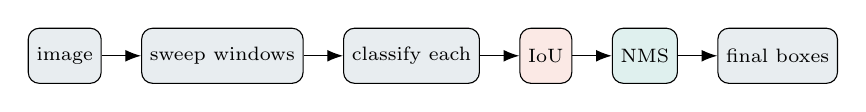
\begin{tikzpicture}[font=\scriptsize,node distance=5mm and 5mm,
      box/.style={draw,rounded corners,fill=coursePrimary!10,minimum height=7mm,inner sep=3pt}]
    \node[box] (img) {image};
    \node[box,right=of img] (win) {sweep windows};
    \node[box,right=of win] (cls) {classify each};
    \node[box,right=of cls,fill=courseAccent!15] (iou) {IoU};
    \node[box,right=of iou,fill=courseGood!15] (nms) {NMS};
    \node[box,right=of nms] (out) {final boxes};
    \draw[-{Latex[length=2mm]}] (img)--(win);
    \draw[-{Latex[length=2mm]}] (win)--(cls);
    \draw[-{Latex[length=2mm]}] (cls)--(iou);
    \draw[-{Latex[length=2mm]}] (iou)--(nms);
    \draw[-{Latex[length=2mm]}] (nms)--(out);
  \end{tikzpicture}
  \end{center}
  \begin{itemize}
    \item Today we build the whole chain by hand; Session 2 replaces ``sweep + classify'' with one CNN.
    \item \term{IoU} and \term{NMS} (the last two boxes) never change --- they survive into every modern detector.
  \end{itemize}
  \keyidea{Keep this chain in view: everything today is one box on this diagram.}
\end{frame}

\begin{frame}{Our running problem, upgraded}
  \begin{columns}[T]
    \begin{column}{0.52\textwidth}
      \begin{center}
      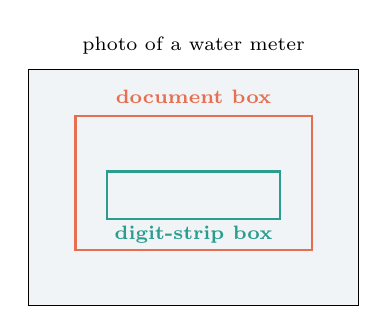
\begin{tikzpicture}[font=\scriptsize]
        \draw[fill=coursePrimary!6] (0,0) rectangle (4.2,3);
        \node at (2.1,3.3) {photo of a water meter};
        % the meter body
        \draw[thick,courseAccent] (0.6,0.7) rectangle (3.6,2.4);
        \node[courseAccent] at (2.1,2.65) {\bfseries document box};
        % the digit strip
        \draw[thick,courseGood] (1.0,1.1) rectangle (3.2,1.7);
        \node[courseGood] at (2.1,0.9) {\bfseries digit-strip box};
      \end{tikzpicture}
      \end{center}
    \end{column}
    \begin{column}{0.48\textwidth}
      \begin{itemize}
        \item Week 13 read an \emph{already-cropped} $8\times8$ digit.
        \item Reality: the phone photo has the meter \emph{somewhere} in the frame.
        \item DocScan must localize the \term{document}, then the \term{digit strip}, \emph{then} read.
      \end{itemize}
      \keyidea{Every idea today plugs into ``find the strip before you read it.''}
    \end{column}
  \end{columns}
\end{frame}

\begin{frame}{A bounding box is just four numbers}
  \begin{columns}[T]
    \begin{column}{0.5\textwidth}
      \begin{itemize}
        \item Corner form: $(x_1,y_1,x_2,y_2)$ --- top-left and bottom-right.
        \item Center form: $(c_x,c_y,w,h)$ --- what detectors predict.
        \item Convert freely: $w=x_2-x_1$, $c_x=x_1+w/2$.
      \end{itemize}
      \begin{mathbox}[Area of a box]
        $\text{area}=(x_2-x_1)\,(y_2-y_1)$
      \end{mathbox}
    \end{column}
    \begin{column}{0.5\textwidth}
      \begin{center}
      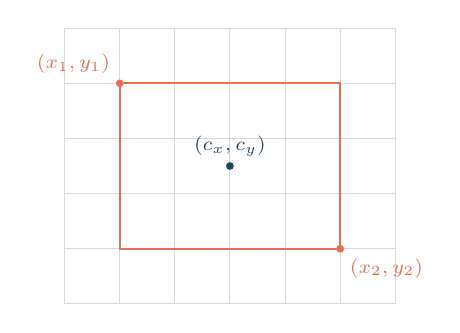
\begin{tikzpicture}[font=\scriptsize,scale=0.7]
        \draw[step=1,gray!30] (0,0) grid (6,5);
        \draw[thick,courseAccent] (1,1) rectangle (5,4);
        \fill[courseAccent] (1,4) circle (2pt) node[above left]{$(x_1,y_1)$};
        \fill[courseAccent] (5,1) circle (2pt) node[below right]{$(x_2,y_2)$};
        \fill[coursePrimary] (3,2.5) circle (2pt) node[above]{$(c_x,c_y)$};
      \end{tikzpicture}
      \end{center}
    \end{column}
  \end{columns}
\end{frame}

\begin{frame}{Localization = regression (one object)}
  \begin{itemize}
    \item Take Week 13's CNN backbone; it already turns an image into features.
    \item Add \emph{two heads} on top of those features:
    \begin{itemize}
      \item a \term{classification head} $\rightarrow$ class scores (softmax, as before);
      \item a \term{box-regression head} $\rightarrow$ 4 numbers $(c_x,c_y,w,h)$.
    \end{itemize}
    \item Train the box head to minimize a regression loss vs. the true box.
  \end{itemize}
  \begin{mathbox}[Box loss (smooth L1 / MSE)]
    $\displaystyle L_{\text{box}}=\sum_{k\in\{c_x,c_y,w,h\}} \big(\hat{k}-k\big)^2$
  \end{mathbox}
  \keyidea{Classification predicts a category; regression predicts numbers. A box is just 4 numbers.}
\end{frame}

\begin{frame}{Box loss, with real numbers}
  Predicted centre-form box $\hat{b}=(30,20,100,40)$, ground truth $b=(32,18,96,44)$.
  \begin{mathbox}[Squared error, term by term]
    $(30{-}32)^2+(20{-}18)^2+(100{-}96)^2+(40{-}44)^2$\\
    $=4+4+16+16=\mathbf{40}$
  \end{mathbox}
  \begin{itemize}
    \item The width/height terms dominate here --- the box is the right place but a little too wide/short.
    \item Gradient descent nudges $(\hat{c}_x,\hat{c}_y,\hat{w},\hat{h})$ to shrink this number, exactly like Week 13.
    \item In practice we use \emph{smooth L1}: squared for small errors, linear for large ones --- robust to outliers.
  \end{itemize}
\end{frame}

\begin{frame}{But real images have \emph{many} objects}
  \begin{itemize}
    \item A single box head can localize \emph{one} object per image.
    \item A meter photo may show the body, several dials, a serial plate\ldots
    \item We do not know \emph{how many} boxes to output in advance.
  \end{itemize}
  \begin{badbox}[The core difficulty of detection]
    Classification has a fixed-size output (10 digit scores). Detection has a \emph{variable} number of outputs --- that is what makes it hard.
  \end{badbox}
\end{frame}

% ==================================================================
\section{The sliding-window idea}
% ==================================================================

\begin{frame}{Sliding windows: brute force, but it works}
  \begin{columns}[T]
    \begin{column}{0.5\textwidth}
      \begin{enumerate}
        \item Pick a window size.
        \item Slide it over the image (like a Week-3 kernel, but bigger).
        \item Run the \term{classifier} on each crop: ``digit strip here? yes/no + score.''
        \item Keep every window that scores high.
      \end{enumerate}
    \end{column}
    \begin{column}{0.5\textwidth}
      \begin{center}
      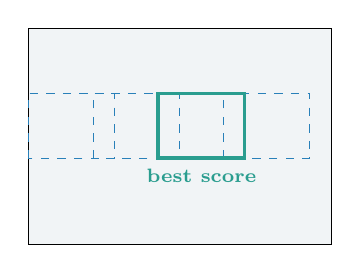
\begin{tikzpicture}[font=\scriptsize,scale=0.55]
        \draw[fill=coursePrimary!6] (0,0) rectangle (7,5);
        \foreach \x in {0,1.5,3,4.5} {
          \draw[courseInfo,dashed] (\x,2) rectangle ++(2,1.5);
        }
        \draw[very thick,courseGood] (3,2) rectangle ++(2,1.5);
        \node[courseGood] at (4,1.6) {\bfseries best score};
      \end{tikzpicture}\\[2pt]
      the window that lands on the object scores highest
      \end{center}
    \end{column}
  \end{columns}
\end{frame}

\begin{frame}{Objects come in many sizes: the image pyramid}
  \begin{itemize}
    \item One window size only finds objects of \emph{that} size.
    \item Fix: shrink the image repeatedly (a \term{pyramid}) and slide the \emph{same} window on each level.
    \item A big object at full size looks small a few levels up --- now the window fits.
  \end{itemize}
  \begin{center}
  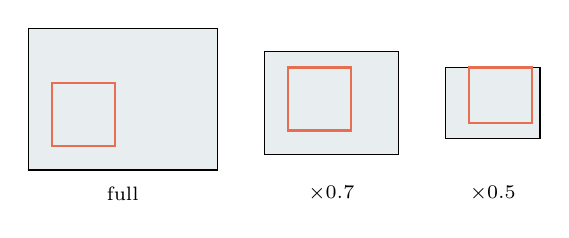
\begin{tikzpicture}[font=\scriptsize]
    \draw[fill=coursePrimary!10] (0,0) rectangle (2.4,1.8); \node at (1.2,-0.3){full};
    \draw[fill=coursePrimary!10] (3,0.2) rectangle (4.7,1.5); \node at (3.85,-0.3){$\times0.7$};
    \draw[fill=coursePrimary!10] (5.3,0.4) rectangle (6.5,1.3); \node at (5.9,-0.3){$\times0.5$};
    \draw[courseAccent,thick] (0.3,0.3) rectangle ++(0.8,0.8);
    \draw[courseAccent,thick] (3.3,0.5) rectangle ++(0.8,0.8);
    \draw[courseAccent,thick] (5.6,0.6) rectangle ++(0.8,0.7);
  \end{tikzpicture}
  \end{center}
  Same coral window, three scales: scale-invariant search for free.
\end{frame}

\begin{frame}{The bill: why brute force hurts}
  \begin{mathbox}[Rough window count]
    $\text{windows}\approx \underbrace{\tfrac{W\,H}{s^2}}_{\text{positions}}\times \underbrace{L}_{\text{scales}}$
  \end{mathbox}
  \begin{itemize}
    \item A $640\times480$ image, stride $s{=}8$, $L{=}5$ scales $\Rightarrow \approx 24{,}000$ classifier calls \emph{per image}.
    \item Add a few aspect ratios and it explodes further.
    \item Slow --- but conceptually it \emph{is} detection. Session 2 makes it fast.
  \end{itemize}
  \begin{goodbox}
    Sliding window is the mental model. Every modern detector is an \emph{efficient} version of this same sweep.
  \end{goodbox}
\end{frame}

\begin{frame}{Now the mess: overlapping detections}
  \begin{columns}[T]
    \begin{column}{0.5\textwidth}
      \begin{itemize}
        \item A good detector fires on \emph{several} nearby windows for one object.
        \item You wanted 1 box; you got 5 overlapping boxes.
        \item We need to (a) measure ``how much do two boxes overlap'' and (b) collapse duplicates.
      \end{itemize}
    \end{column}
    \begin{column}{0.5\textwidth}
      \begin{center}
      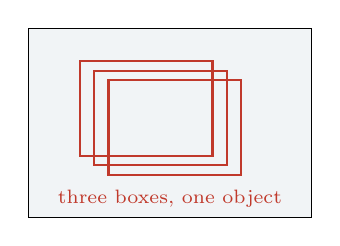
\begin{tikzpicture}[font=\scriptsize,scale=0.6]
        \draw[fill=coursePrimary!6] (0,0) rectangle (6,4);
        \draw[courseBad,thick] (1.4,1.1) rectangle (4.2,3.1);
        \draw[courseBad,thick] (1.7,0.9) rectangle (4.5,2.9);
        \draw[courseBad,thick] (1.1,1.3) rectangle (3.9,3.3);
        \node[courseBad] at (3,0.4){three boxes, one object};
      \end{tikzpicture}
      \end{center}
    \end{column}
  \end{columns}
  \keyidea{The fix is two ideas: \term{IoU} (measure overlap) and \term{NMS} (keep the best, drop the rest).}
\end{frame}

% ==================================================================
\section{IoU: measuring overlap}
% ==================================================================

\begin{frame}{Intersection over Union (IoU)}
  \begin{columns}[T]
    \begin{column}{0.55\textwidth}
      \begin{itemize}
        \item \term{IoU} $=\dfrac{\text{area of overlap}}{\text{area of union}}$.
        \item $0$ = no overlap, $1$ = identical boxes.
        \item It is how we score a predicted box against the truth, \emph{and} how NMS spots duplicates.
      \end{itemize}
      \begin{mathbox}[Union without double-counting]
        $\text{union}=A_1+A_2-\text{intersection}$
      \end{mathbox}
    \end{column}
    \begin{column}{0.45\textwidth}
      \begin{center}
      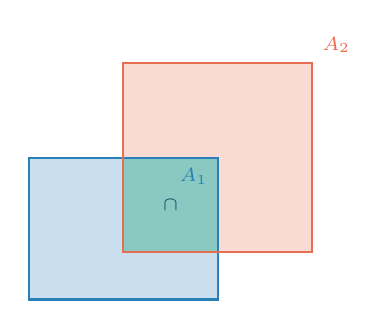
\begin{tikzpicture}[font=\scriptsize,scale=0.6]
        \fill[courseInfo!25] (1,1) rectangle (5,4);
        \fill[courseAccent!25] (3,2) rectangle (7,6);
        \fill[courseGood!55] (3,2) rectangle (5,4);
        \draw[courseInfo,thick] (1,1) rectangle (5,4) node[below left,courseInfo]{$A_1$};
        \draw[courseAccent,thick] (3,2) rectangle (7,6) node[above right,courseAccent]{$A_2$};
        \node[coursePrimary] at (4,3){$\cap$};
      \end{tikzpicture}
      \end{center}
    \end{column}
  \end{columns}
\end{frame}

\begin{frame}{IoU, by hand}
  Boxes in $(x_1,y_1,x_2,y_2)$: $A=(1,1,5,4)$, $B=(3,2,7,6)$.
  \begin{columns}[T]
    \begin{column}{0.5\textwidth}
      \begin{mathbox}[Overlap rectangle]
        $x$: $[\max(1,3),\min(5,7)]=[3,5]\Rightarrow 2$\\
        $y$: $[\max(1,2),\min(4,6)]=[2,4]\Rightarrow 2$\\
        $\text{inter}=2\times2=\mathbf{4}$
      \end{mathbox}
    \end{column}
    \begin{column}{0.5\textwidth}
      \begin{mathbox}[Areas and IoU]
        $A_1=(5{-}1)(4{-}1)=12$\\
        $A_2=(7{-}3)(6{-}2)=16$\\
        $\text{union}=12+16-4=24$\\
        $\text{IoU}=\dfrac{4}{24}=\mathbf{0.167}$
      \end{mathbox}
    \end{column}
  \end{columns}
  \vspace{2pt}
  Overlap width/height clamp at $0$: if the ranges do not cross, intersection is $0$, not negative.
\end{frame}

\begin{frame}{Reading IoU numbers}
  \begin{center}
  \begin{tabular}{@{}ll@{}}
    \toprule
    \textbf{IoU} & \textbf{Meaning} \\
    \midrule
    $0$        & boxes do not touch \\
    $0.1$--$0.3$ & slight overlap; probably different objects \\
    $0.5$      & the classic ``a hit'' threshold for evaluation \\
    $0.7$--$0.9$ & tight, well-aligned prediction \\
    $1.0$      & pixel-perfect identical boxes \\
    \bottomrule
  \end{tabular}
  \end{center}
  \begin{goodbox}
    IoU $\ge 0.5$ is the community default for ``correct enough.'' Stricter tasks demand $0.75$.
  \end{goodbox}
\end{frame}

\begin{frame}{An IoU gallery}
  \begin{center}
  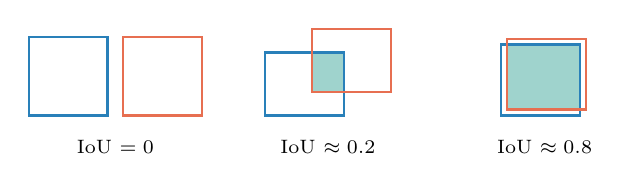
\begin{tikzpicture}[font=\scriptsize,scale=0.5]
    % case 1: disjoint
    \draw[courseInfo,thick] (0,0) rectangle (2,2);
    \draw[courseAccent,thick] (2.4,0) rectangle (4.4,2);
    \node at (2.2,-0.8) {IoU $=0$};
    % case 2: partial
    \begin{scope}[xshift=6cm]
      \fill[courseGood!45] (1.2,0.6) rectangle (2,1.6);
      \draw[courseInfo,thick] (0,0) rectangle (2,1.6);
      \draw[courseAccent,thick] (1.2,0.6) rectangle (3.2,2.2);
      \node at (1.6,-0.8) {IoU $\approx0.2$};
    \end{scope}
    % case 3: tight
    \begin{scope}[xshift=12cm]
      \fill[courseGood!45] (0.15,0.15) rectangle (2,1.8);
      \draw[courseInfo,thick] (0,0) rectangle (2,1.8);
      \draw[courseAccent,thick] (0.15,0.15) rectangle (2.15,1.95);
      \node at (1.1,-0.8) {IoU $\approx0.8$};
    \end{scope}
  \end{tikzpicture}
  \end{center}
  \begin{itemize}
    \item Left: separate objects. Middle: partial overlap --- likely two things. Right: near-perfect box.
    \item Green shows the intersection; IoU grows as the two boxes line up.
  \end{itemize}
  \keyidea{Train IoU-reading by eye: it is the number you will debug detectors with most.}
\end{frame}

% ==================================================================
\section{NMS: keeping the best box}
% ==================================================================

\begin{frame}{Non-Maximum Suppression (NMS)}
  \begin{columns}[T]
    \begin{column}{0.54\textwidth}
      The greedy recipe, per class:
      \begin{enumerate}
        \item Sort all boxes by score, high $\to$ low.
        \item Take the top box; \emph{keep} it.
        \item Remove every remaining box whose IoU with it exceeds a threshold $\tau$ (e.g. $0.5$).
        \item Repeat with the next surviving box until none remain.
      \end{enumerate}
    \end{column}
    \begin{column}{0.46\textwidth}
      \begin{infobox}[Why ``non-maximum''?]
        For each cluster of overlapping boxes we keep only the \emph{maximum}-scoring one and \emph{suppress} the rest. Duplicates gone; distinct objects kept.
      \end{infobox}
    \end{column}
  \end{columns}
\end{frame}

\begin{frame}{NMS, by hand}
  Three boxes, threshold $\tau=0.5$:
  \begin{center}
  \begin{tabular}{@{}lccl@{}}
    \toprule
    \textbf{Box} & \textbf{Score} & \textbf{IoU with kept} & \textbf{Action} \\
    \midrule
    B1 & 0.90 & --- & \textbf{keep} (highest) \\
    B2 & 0.80 & $0.70$ vs B1 & suppress ($>\tau$) \\
    B3 & 0.75 & $0.10$ vs B1 & \textbf{keep} (different object) \\
    \bottomrule
  \end{tabular}
  \end{center}
  \begin{itemize}
    \item Start with B1 (top score). B2 overlaps it heavily $\Rightarrow$ drop as a duplicate.
    \item B3 barely overlaps $\Rightarrow$ it is a \emph{second} object; keep it.
    \item Output: \{B1, B3\}. Three noisy boxes became two clean detections.
  \end{itemize}
\end{frame}

\begin{frame}{Choosing the NMS threshold}
  \begin{columns}[T]
    \begin{column}{0.5\textwidth}
      \begin{badbox}[$\tau$ too low ($0.2$)]
        Aggressive: two \emph{real} objects that stand close (two dials) get merged into one --- missed detections.
      \end{badbox}
    \end{column}
    \begin{column}{0.5\textwidth}
      \begin{badbox}[$\tau$ too high ($0.9$)]
        Timid: duplicate boxes survive --- one meter reported three times.
      \end{badbox}
    \end{column}
  \end{columns}
  \vspace{2pt}
  \keyidea{$\tau\approx0.5$ is the usual compromise. Crowded scenes need care --- or ``Soft-NMS,'' which \emph{lowers} scores instead of hard-dropping.}
\end{frame}

% ==================================================================
\section{In-class exercise}
% ==================================================================

\begin{frame}{\faPen~In-class exercise (10 min)}
  \begin{infobox}[Compute overlap and clean up]
  \end{infobox}
  \begin{enumerate}
    \item Box $P=(0,0,4,4)$ and $Q=(2,2,6,6)$. Compute the intersection area, union area, and IoU.
    \item Two boxes do not overlap at all. What is their IoU, and why can't intersection be negative?
    \item You have boxes with scores $0.95, 0.9, 0.6$; the first two have IoU $0.8$, the third has IoU $0.05$ with both. Run NMS at $\tau=0.5$: what survives?
    \item A $600\times400$ image, stride $10$, $4$ scales. Roughly how many sliding windows?
  \end{enumerate}
\end{frame}

\begin{frame}{\faPen~Debrief}
  \begin{itemize}
    \item (1) inter $=2\times2=4$; areas $16$ and $16$; union $=16+16-4=28$; IoU $=4/28\approx0.14$.
    \item (2) IoU $=0$. Overlap width/height are \emph{clamped} at $0$ --- non-touching ranges give $0$, never a negative area.
    \item (3) Keep $0.95$; suppress $0.9$ (IoU $0.8>\tau$); keep $0.6$ (IoU $0.05$). Survivors: $\{0.95,\,0.6\}$.
    \item (4) $\tfrac{600\cdot400}{10^2}\times4 = 2400\times4 = 9600$ windows --- and that's just one aspect ratio.
  \end{itemize}
  \keyidea{You can now score a box against the truth and clean a pile of boxes into final detections.}
\end{frame}

% ==================================================================
\section{Wrap-up}
% ==================================================================

\begin{frame}{Common pitfalls}
  \begin{badbox}[Watch out]
    \begin{itemize}
      \item Forgetting to \emph{clamp} the overlap: negative width/height must become $0$, not a phantom area.
      \item Double-counting in the union --- subtract the intersection exactly once.
      \item Running NMS \emph{across} classes: suppress within a class, or a meter kills a nearby dial.
      \item Treating a low-IoU neighbour as a duplicate --- it is often a second, real object.
    \end{itemize}
  \end{badbox}
\end{frame}

\begin{frame}{Good habits}
  \begin{goodbox}
    \begin{itemize}
      \item Decide your box format ($x_1y_1x_2y_2$ vs centre) \emph{once} and convert at the edges.
      \item Sanity-check IoU on two identical boxes ($=1$) and two disjoint boxes ($=0$).
      \item Keep NMS per class, and log how many boxes it removes --- a great debugging signal.
    \end{itemize}
  \end{goodbox}
\end{frame}

\begin{frame}{What you can already do}
  \begin{itemize}
    \item State the difference between classification, localization, and detection.
    \item Describe a box as 4 numbers and localization as regression on those numbers.
    \item Explain the sliding-window sweep and why the image pyramid handles scale.
    \item Compute IoU by hand and run NMS on a small set of boxes.
  \end{itemize}
\end{frame}

\begin{frame}{Next session}
  \begin{alertblock}{Session 2 --- from brute force to a real detector}
    \begin{itemize}
      \item Why sliding windows are too slow, and how \term{region proposals} trimmed the search.
      \item The leap to \term{single-shot} detectors (\term{YOLO}): one grid, one forward pass.
      \item \term{Anchor boxes}, the objectness/confidence score, and the output tensor.
      \item Measuring a detector honestly with \term{precision/recall} and \term{mAP} --- then the DocScan deliverable.
    \end{itemize}
  \end{alertblock}
  \emph{Bring today's IoU and NMS firmly in mind --- every modern detector leans on both.}
\end{frame}

\begin{frame}[standout]
  Detection = ``what'' plus ``where.''\\[4pt]
  \normalsize Today: boxes, the sliding-window sweep, IoU to score overlap, NMS to keep the best. Next: make it fast.
\end{frame}

\end{document}
